\documentclass[
ngerman,
]{tudaexercise}

\usepackage[english]{babel}
\usepackage{amsmath}
\usepackage{amsthm}
\usepackage{amssymb}
\usepackage{mathtools}
\usepackage{array}
\usepackage{gauss}
\usepackage{graphicx}
\usepackage{lipsum}% For example text
\usepackage{listings}
\usepackage{float}
\graphicspath{ {./images/} }
\newcommand{\sni}{\sum_{i=1}^{n}}

\begin{document}
	
	\title[Uebung]{SML: Exercise 2}
	\author{Rinor Cakaj, Patrick Nowak}
	\term{Summer Term 2020}
	\sheetnumber{1}
	
	\maketitle

	\begin{task}{Bayesian Decision Theory}
		In this exercise, we consider data generated by a mixture of two Gaussian distributions with parameters $\{\mu_1, \sigma_1\}$ and $\{\mu_2, \sigma_2\}$. Each Gaussian represents a class labeled C1 and C2, respectively.
		\begin{subtask}
			The bayesian decision theory finds the a-posteriori probability (posterior) of a class $C_k$ given a observation (feature) $x$ by using the Bayes Theorem
			\begin{align*}
			p(C_k | x) = \frac{p(x|C_k)p(C_k)}{p(x)}.
			\end{align*}
			The goal of bayesian decision theory is to minimize the misclassification rate. Let $C_1, C_2$ be two cases. The condition which holds at the optimal decision boundary is
			\begin{align*}
			p(C_1 | x ) = p (C_2 | x).
			\end{align*}
			We decide $C_1$ if 
			\begin{align*}
			p(C_1 | x) > p(C_2 | x).
			\end{align*}
		\end{subtask}
		\begin{subtask}
			Let both classes $C_1$ and $C_2$ have equal probabilities $p(C_1) = p(C_2)$ and the same variance $\sigma_1, \sigma_2$. In the following we will derive the decision boundary $x^*$ analytically as a function of two means $\mu_1, \mu_2$.
			\begin{align*}
			p(C_1 | x) &= p(C_2 | x) \\
			\frac{p(x | C_1) p(C_1)}{p(x)} &= \frac{p(x | C_2) p(C_2)}{p(x)} \quad | \div p(C_1) \quad | \cdot p(x) \\
			p(x | C_1) &= p(x |C_2) \\
			\frac{1}{\sqrt{2 \pi} \sigma_1} \exp \left( -\frac{(x- \mu_1)^2}{2 \sigma_1^2} \right) &= \frac{1}{\sqrt{2 \pi} \sigma_2} \exp \left( -\frac{(x- \mu_2)^2}{2 \sigma_2^2} \right) \quad | \div \frac{1}{\sqrt{2 \pi} \sigma_1} \quad | \ln() \\
			-\frac{(x- \mu_1)^2}{2 \sigma_1^2} &= -\frac{(x- \mu_2)^2}{2 \sigma_2^2} \quad | \cdot 2 \sigma_1^2 \\
			(x- \mu_1)^2 &= (x - \mu_2)^2 \\
			x^2 - 2x\mu_1 + \mu_1^2 &= x^2 - 2x\mu_2 + \mu_2^2 \\
			\mu_1^2 - \mu_2^2 &= (-2 \mu_2 + 2 \mu_1)x \\
			x &= \frac{\mu_1^2 - \mu_2^2}{-2 \mu_2 + 2 \mu_1}\\
			x &= \frac{\mu_1 + \mu_2}{2}
			\end{align*}
		\end{subtask}
		\begin{subtask}
			Let $\mu_1 < 0, \mu_1 = 2\mu_2, \sigma_1 = \sigma_2$ and $p(C_1) = p(C_2)$. The misclassification of a sample $x \in C_2$ as a class $C_1$ should be four times more expensive than the opposite. Clearly our boundary will change in such a way, that we classify $x$ more often as in class $C_2$ then in class $C_1$. In the following we will derive the boundary analytically.
			\begin{align*}
			R(\alpha_1 | x) = 4 p(C_2 | x)\\
			R(\alpha_2 | x) = p(C_1 | x)
			\end{align*}
			We will get the decision boundary by looking at
			\begin{align*}
			R(\alpha_2 | x) &= R( \alpha_1 | x) \\
			p(C_1 | x) &= 4p(C_2 | x) \text{ same computations as in 1.1b) } \\
			p(x | C_1) &= p(x | C_2) \\
			\frac{1}{\sqrt{2 \pi} \sigma_1} \exp \left( -\frac{(x- \mu_1)^2}{2 \sigma_1^2} \right) &= \frac{4}{\sqrt{2 \pi} \sigma_2} \exp \left( -\frac{(x- \mu_2)^2}{2 \sigma_2^2} \right) \quad | \div \frac{1}{\sqrt{2 \pi} \sigma_1} \quad | \ln() \\
			-\frac{(x- \mu_1)^2}{2 \sigma_1^2} &= \ln(4) -\frac{(x- \mu_2)^2}{2 \sigma_2^2} \quad | \cdot 2 \sigma_1^2 \\
			-(x - \mu_1)^2 &= 2 \sigma_1^2 \ln(4) - (x - \mu_2)^2 \\
			-x^2 + 2 \mu_1 x - \mu_1^2 &= 2 \sigma_1^2 \ln(4) - x^2 + 2x \mu_2 - \mu_2^2 \\
			2 \mu_1x - 2\mu_2x &= 2 \sigma_1^2 \ln(4) - \mu_2^2 - \mu_1^2 \\
			x &= \frac{2 \sigma_1^2 \ln(4) - \mu_2^2 + \mu_1^2}{\mu_1} \\
			x &= \frac{2 \sigma_1^2 \ln(4) + 3\mu_2^2}{\mu_1}
			\end{align*}
		\end{subtask}
	\end{task}
	
	\begin{task}{Density Estimation}
		We are given data C1 and C2, which we suppose to be generated by 2D-Gaussians with parameters ${\mu_1,\Sigma_1}$ and ${\mu_2,\Sigma_2}$, respectively.
		\begin{subtask}
	Assume we are given iid. datapoints $x_i, i=1,..,n$ which are generated by a 2D-Gaussian. Following the max-likelihood principle, we maximize the log-likelihood function
	\begin{align*}
	l(\mu,\Sigma,x_1,...,x_n)=\ln(\prod_{i=1}^n p(x_i|\mu,\Sigma))=\sni\ln(p(x_i|\mu,\Sigma))
	\end{align*}
	for the Gaussian probability density
	\begin{align}\label{gaussian} p(x|\mu,\Sigma)=\frac{1}{\sqrt{(2\pi)^2|\Sigma|}}\exp\left( -\frac{1}{2}(x-\mu)^T\Sigma^{-1}(x-\mu)\right)\;.
	\end{align}
	We receive
	\begin{align}
	l(\mu,\Sigma):=l(\mu,\Sigma,x_1,...,x_n)&=\sni\left( -\ln(2\pi)-\frac{1}{2}ln(|\Sigma|)-\frac{1}{2}(x_i-\mu)^T\Sigma^{-1}(x_i-\mu)\right) \\
	&=-n \ln(2\pi)-\frac{n}{2}ln(|\Sigma|)-\frac{1}{2}\sni (x_i-\mu)^T\Sigma^{-1}(x_i-\mu)\;\;.\label{lfkt}
	\end{align}
	We compute the derivatives w.r.t. $\mu$ and $\Sigma$ and set them equal to zero. This yields
	\begin{align*}
	\frac{d}{d\mu}l(\mu,\Sigma,x_1,...,x_n)&=\frac{d}{d\mu}\; -\frac{1}{2}\sni (x_i-\mu)^T\Sigma^{-1} (x_i-\mu)\\ &= -\sni \frac{d}{d\mu}\frac{1}{2}(x_i-\mu)^T\Sigma^{-1} (x_i-\mu)\;\;.
	\end{align*}
	Using the matrix identity $\frac{d}{dw}\frac{w^T Aw}{dw}=2Aw$ which holds if $w$ does not depend on $A$ and if $A$ is symmetric, we get (with $w=(x-\mu), dw=-d\mu$)
	\begin{align*}
	0&\stackrel{!}{=}\frac{d}{d\mu}l(\mu,\Sigma,x_1,...,x_n)\\
	0&\stackrel{!}{=}-\sni \Sigma^{-1}(x_i-\mu)	\;\;.
	\end{align*}
	Finally, we use that $\Sigma^{-1}$ is positive definite, so we can leave it out here and get
	\begin{align*}
	0&\stackrel{!}{=}n\mu-\sni x_i\;\;,
	\end{align*}
	which is solved for the MLE-estimate
	\begin{align}\label{mean}
	\hat{\mu}&=\frac{1}{n}\sni x_i\;\;.
	\end{align}
	Secondly, we need to compute the derivative w.r.t $\Sigma$. To do that, we will need some results from mathematical classes. The following is used without prove:
	\begin{itemize}
		\item Cyclic permutations of a matrix product do not change the trace of it:\begin{align*}
		tr\left[ ABC\right] = tr\left[ CAB\right] 
		\end{align*}
		\item The trace of a scalar is the scalar itself. In particular: the result of a quadratic form $x^T Ax$ is a scalar, such that:\begin{align*}
		x^T Ax=tr\left[ x^TAx\right] =tr\left[ x^TxA\right] 
		\end{align*}
		\item $\frac{d}{dA}tr\left[ AB\right] =B^T$
		\item $\frac{d}{dA}\ln|A|=A^{-T}$
	\end{itemize}
	As a first result of these assumptions, we can show, that\begin{align*}
	\frac{d}{dA}x^T Ax=\frac{d}{dA}tr\left[ x^T xA\right] =\left[ xx^T\right] ^T=xx^T\;.
	\end{align*} 
	We now got the tools to re-write the log-likelihood function in (\ref{lfkt}) to
	\begin{align*}
	l(\mu,\Sigma)&=-n\ln(2\pi)-\frac{n}{2}ln(|\Sigma|)-\frac{1}{2}\sni (x_i-\mu)^T\Sigma^{-1}(x_i-\mu)\\&=C+\frac{n}{2}ln(|\Sigma^{-1}|)-\frac{1}{2}\sni tr\left[ (x_i-\mu)(x_i-\mu)^T \Sigma^{-1}\right] \\&=C+\frac{n}{2}ln(|\Sigma^{-1}|)-\frac{1}{2}\sni tr\left[\Sigma^{-1} (x_i-\mu)(x_i-\mu)^T \right] 
	\end{align*}
	for a constant C. Where in the last step we used that $AB=BA$ for symmetric matrices $A, B$. Taking the derivative w.r.t $\Sigma^{-1}$ yields
	\begin{align*}
	\frac{d}{d\Sigma^{-1}}l(\mu,\Sigma)=\frac{n}{2}\Sigma^T-\frac{1}{2}\sni(x_i-\mu)(x_i-\mu)^T
	\end{align*}
	and plugging in $\hat{\mu}$ as an estimation of $\mu$ and setting equal to zero finally gives us
	\begin{align*}
	0&\stackrel{!}{=}\frac{d}{d\Sigma^{-1}}l(\hat{\mu},\Sigma)\\
	0&\stackrel{!}{=}\frac{n}{2}\Sigma^T-\frac{1}{2}\sni(x_i-\hat{\mu})(x_i-\hat{\mu})^T
	\end{align*}
	which is solved for the (biased) MLE estimate
	\begin{align}\label{bsigma}
	\tilde{\Sigma}=\frac{1}{n}\sni (x_i-\hat{\mu})(x_i-\hat{\mu})^T
	\end{align}
\end{subtask}
	\begin{subtask}
		We compute the prior probabilities of C1 and C2, using the following python code. We read the number of data points in each class and divide it by the sum of total data points in both classes.
		\begin{lstlisting}[language=Python]
	import numpy as np
	
	link1="../hw2/dataSets/densEst1.txt"
	link2="../hw2/dataSets/densEst2.txt"
	
	def get_lengths():
		l1=0;
		l2=0;
		for line in open(link1):
			l1=l1+1
		for line2 in open(link2):
			l2=l2+1
		return (l1,l2)    
	
	def get_priors(l1,l2):
		p_C1=l1/(l1+l2)
		p_C2=l2/(l1+l2)
		return(p_C1,p_C2)
		\end{lstlisting}
		Calling
		\begin{lstlisting}[language=Python]
	lengths=get_lengths()
	print(get_priors(lengths[0],lengths[1]))
		\end{lstlisting}
		we get the following results for the prior probabilities: p(C1)=0.239 and p(C2)=0.761 .
		\end{subtask}
	\begin{subtask}
		Having a data set $X$ and an estimator $\hat{\theta}$ on the true parameter $\theta$, we define the bias of an estimator as the expected deviation from the true parameter. We get the formula\begin{align*}bias(\hat{\theta})=\mathbb{E}_X\left[ \hat{\theta}(X)-\theta\right] 
		\end{align*} We call an estimator unbiased iff $bias(\hat{\theta})=0$ and biased otherwise.\\From the lecture we know that the MLE of the mean of a Gaussian is unbiased, but the MLE of the variance of a Gaussian is biased. In fact, an unbiased estimator on the variance would be the sample covariance matrix \begin{align}\label{sigma}
\hat{\Sigma}=\frac{1}{n-1}\sni(x_i-\hat{\mu})(x_i-\hat{\mu})^T \;.
		\end{align}
		To calculate the conditional distribution densities $p(x|C_i)$ we need to estimate the underlying parameters $\mu_i$ and $\Sigma_i$. For both classes we use the MLE-estimate of the mean, which is unbiased and calculated like in (\ref{mean}). We compute the biased MLE-estimate $\tilde{\Sigma}$ for the variance via (\ref{bsigma}) and the unbiased estimate $\hat{\Sigma}$ via (\ref{sigma}). We wrote the following python code
		\begin{lstlisting}[language=Python]
		def extract_data(t):
			a=np.empty((0,2),float)
			for line in t:
				v=np.array([[line.split()[0],line.split()[1]]],float)
				a=np.append(a,v,axis=0)
			return a
		
		def get_mean_estimation(points):
			m=np.zeros(2)
			m[0]=sum(points[:,0])
			m[1]=sum(points[:,1])
			m=m/len(points)
			return m
		
		def get_biased_var_estimation(mean_est,points):
			l=points-mean_est
			s=np.zeros((2,2))
			for line in l:
				s=s+np.outer(line,line)
			s=s/len(l)
		return s
		
		def get_unbiased_var_estimation(mean_est,points):
			l=points-mean_est
			s=np.zeros((2,2))
			for line in l:
				s=s+np.outer(line,line)
			s=s/(len(l)-1)
		return s
		
		def print_results(link):
			a=extract_data(open(link))
			mean=get_mean_estimation(a)
			print("mean=",mean)
			sigma=get_unbiased_var_estimation(mean,a)
			print("biased_Sigma=",get_biased_var_estimation(mean,a))
			print("sigma=",sigma)
		\end{lstlisting}
		which gives us the results for class C1
		\begin{lstlisting}
		print_results(link1)
		
		mean= [-0.70681374 -0.81343083]
		biased_Sigma= [[9.01952586 2.67287085]
				[2.67287085 3.59633965]]
		sigma= [[9.05742302 2.6841014 ]
			[2.6841014  3.61145033]]
		\end{lstlisting}
		and for class C2
		\begin{lstlisting}
		print_results(link2)
		
		mean= [3.98534252 3.98438364]
		biased_Sigma= [[4.1753815  0.02758324]
			[0.02758324 2.75296323]]
		sigma= [[4.18087542 0.02761954]
			[0.02761954 2.75658555]]
		\end{lstlisting}
		Transfered to the notation we introduced earlier, we get $\hat{\mu_1}=\begin{pmatrix}
		-0.71\\-0.81
		\end{pmatrix}$ with $\tilde{\Sigma_1}=\begin{pmatrix}
		9.02 & 2.67\\2.67 & 3.6
		\end{pmatrix}$ or with the unbiased $\hat{\Sigma_1}=\begin{pmatrix}9.06&2.68\\2.68&3.61
		\end{pmatrix}$ for C1.\\ And $\hat{\mu_2}=\begin{pmatrix}
		3.99\\3.98
		\end{pmatrix}$ with $\tilde{\Sigma_2}=\begin{pmatrix}
		4.18&0.03\\0.03&2.75
		\end{pmatrix}$ or with the unbiased $\hat{\Sigma_2}=\begin{pmatrix}		4.18&0.03\\0.03&2.76
		\end{pmatrix}$ for C2.\\
		We can now just plug in into formula (\ref{gaussian}) to get \\for the biased estimate $p(x|C_i)=p(x|\hat{\mu_i},\tilde{\Sigma_i})$ \\and for the unbiased $p(x|C_i)=p(x|\hat{\mu_i},\hat{\Sigma_i})$, where the right hand sides are given like in (\ref{gaussian}).
	\end{subtask}
\begin{subtask}
	Using the unbiased estimates $p(x|C_i)=p(x|\hat{\mu_i},\hat{\Sigma_i})$ from last task, for each class we plot the Gaussian in a single graph with the data points: Therefore we added 2 new functions to our code:
	\begin{lstlisting}[language=Python]
		def gaussian(x,mu,detsigma,sigmainv):
			z=np.array(x-mu)
			enum=np.exp(-0.5*np.dot(np.dot(z,sigmainv),np.transpose(z)))
			denom=np.sqrt(np.power(2*np.pi,len(x))*detsigma)
			return enum/denom
		
		def plot(link):
			a=extract_data(open(link))
			mean=get_mean_estimation(a)
			print("mean=",mean)
			sigma=get_unbiased_var_estimation(mean,a)
			print("biased_Sigma=",get_biased_var_estimation(mean,a))
			print("sigma=",sigma)
			detsigma=np.linalg.det(sigma)
			sigmainv=np.linalg.inv(sigma)
			x=np.linspace(min(a[:,0]),max(a[:,0]),300)
			y=np.linspace(min(a[:,1]),max(a[:,1]),300)
			X,Y=np.meshgrid(x,y)
			Z=np.empty_like(X)
			i=0
			while i<len(X):
				j=0
				while j<len(Y):
					xy=np.array([X[i,j],Y[i,j]])
					ergb=gaussian(xy,mean,detsigma,sigmainv)
					Z[i,j]=ergb
					j=j+1
				i=i+1
			plt.contourf(X,Y,Z,25)
			plt.colorbar()
			plt.scatter(a[:,0],a[:,1],alpha=1,c="white",s=0.8)
			return
	\end{lstlisting}
	Calling "plot(link1)" gives us Figure 1 and "plot(link2)" gives Figure 2.
	\begin{figure}[H]
	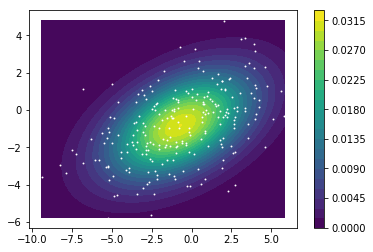
\includegraphics[width=0.8\textwidth]{d1plot.png}
	\caption{Gaussian ($\hat{\mu_1},\hat{\Sigma_1}$) and data points C1 in white}
	\end{figure}
	\begin{figure}[H]
	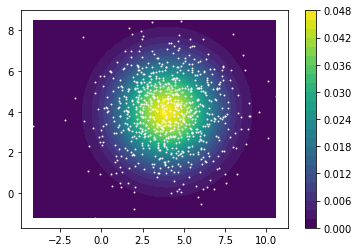
\includegraphics[width=0.8\textwidth]{d2plot.png}
	\caption{Gaussian ($\hat{\mu_2},\hat{\Sigma_2}$) and data points C2 in white}
\end{figure}
\end{subtask}\noindent
\begin{subtask}
	We are interested in $p(C_i|x)$. From Bayes' rule we know that this equals\begin{align*}
		p(C_i|x)=\frac{p(x|C_i)p(C_i)}{\sum_j p(x|C_j)p(C_j)}
	\end{align*}
	which helps us a lot because we calculated all terms occuring in the right hand side. We add two more functions to our code:
	\begin{lstlisting}[language=Python]
		def postplot(link):
			g=extract_data(open(link3))
			a=extract_data(open(link))
			prior=len(a)/len(g)
			mean=get_mean_estimation(a)
			sigma=get_unbiased_var_estimation(mean,a)
			detsigma=np.linalg.det(sigma)
			sigmainv=np.linalg.inv(sigma)
			x=np.linspace(min(g[:,0]),max(g[:,0]),300)
			y=np.linspace(min(g[:,1]),max(g[:,1]),300)
			X,Y=np.meshgrid(x,y,sparse=False)
			Z=np.empty_like(X)
			i=0
			while i<len(X):
				j=0
				while j<len(Y):
					xy=np.array([X[i,j],Y[i,j]])
					ergb=prior*gaussian(xy,mean,detsigma,sigmainv)
					Z[i,j]=ergb
					j=j+1
				i=i+1
			return [X,Y,Z,prior]
		
		def actual_plotting():
			X,Y,Z1,p1=postplot(link1)
			Z2,p2=postplot(link2)[2:4]
			S=np.add(Z1,Z2)
			Z1neu=np.divide(Z1,S)
			Z2neu=np.divide(Z2,S)
			plt.contour(X,Y,Z1,10)
			plt.contour(X,Y,Z2,10)
			plt.title("likelihood x prior")
			plt.figure()
			plt.contour(X,Y,Z1neu,10)
			plt.colorbar()
			plt.title("p(C1|x)")
			plt.figure()
			plt.contour(X,Y,Z2neu,10)
			plt.colorbar()
			plt.title("p(C2|x)")
			plt.figure()
			dec=np.greater(Z1neu,Z2neu)
			plt.scatter(X,Y,dec)
			plt.title("blue=decideC1, white=decideC2") 
			j=0
			mpoints=np.empty(shape=[0,2])
			while j<len(X):
				i=0
				while i<len(Y):
					if not dec[i,j]:
						xy=np.array([[X[i,j],Y[i,j]]])
						mpoints=np.append(mpoints,xy,axis=0)
						break
					i=i+1
				j=j+1
			plt.figure()
			plt.scatter(mpoints[:,0],mpoints[:,1],s=0.5)
			plt.title("decision boundary") 
			plt.figure()
			plt.contour(X,Y,Z1,10)
			plt.contour(X,Y,Z2,10)
			plt.scatter(mpoints[:,0],mpoints[:,1],s=0.5)
    			plt.title("likelihood x prior and decbound")

			return
	\end{lstlisting}
	Where in link3 we stored a link to a .txt file containing all data from C1 and C2 combined. This can be generated by executing
	\begin{lstlisting}[language=Python]
		def merge_txt(inp):
			with open('../hw2/dataSets/densEstCombined.txt', 'w') as outfile:
				for fname in inp:
					with open(fname) as infile:
						for line in infile:
							outfile.write(line)
			return
	\end{lstlisting}
	once, or just do it by hand. Calling actual\_plotting() then gives us the following results:
	\begin{figure}[H]
		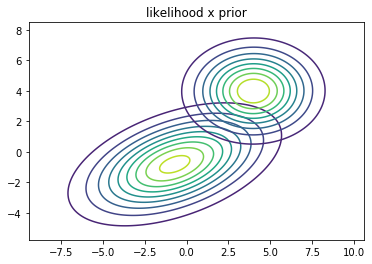
\includegraphics{likexprior.png}
	\end{figure}
\begin{figure}[H]
		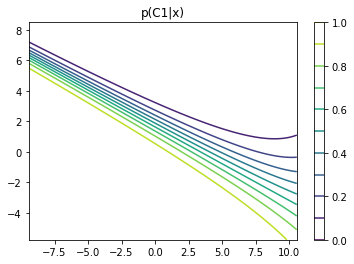
\includegraphics{pc1x.png}
\end{figure}
\begin{figure}[H]
	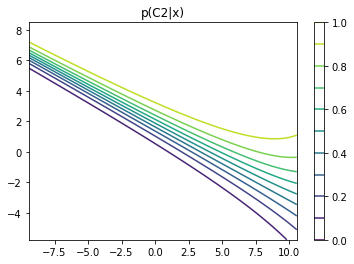
\includegraphics{pc2x.png}
\end{figure}
\begin{figure}[H]
	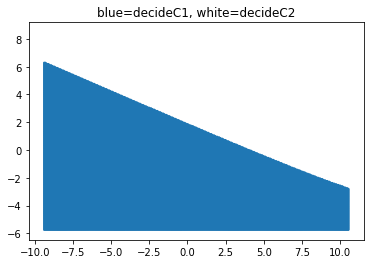
\includegraphics{dec1.png}
\end{figure}
\begin{figure}[H]
	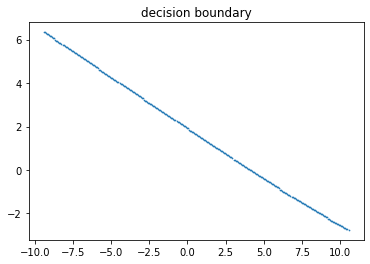
\includegraphics{dec2.png}
\end{figure}
\begin{figure}[H]
	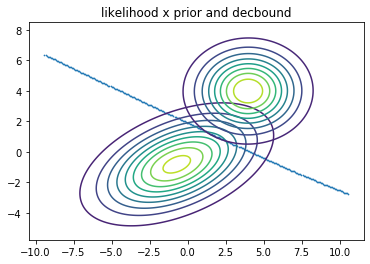
\includegraphics{dec3.png}
\end{figure}
	\end{subtask}
	\end{task}
\begin{task}{Non-parametric Density Estimation}
	\begin{subtask}{Histogram}
		Given training data, we plot histograms with different binsizes. We therefore wrote a python function that plots a histogram given data and a binsize:
		\begin{lstlisting}[language=Python]
	def histogram(data, bin_size):
		bins = np.arange(min(data), max(data) + bin_size, bin_size)
		hist = np.zeros((len(bins),2))
		hist[:,0] = bins
			for i in range(len(hist)):
				for j in range(len(data)):
					if hist[i,0] <= data[j] < hist[i+1,0]:
						hist[i,1] = hist[i,1] + 1
					hist[:,0] = hist[:,0] + 0.5 * bin_size

		plt.bar(hist[:,0], hist[:,1], color="red", width=bin_size)
		plt.title("bin size="+ str(bin_size))       
		plt.show()
		\end{lstlisting}
		Calling the function for different binsizes with our training data gives us:
		\begin{figure}[H]
		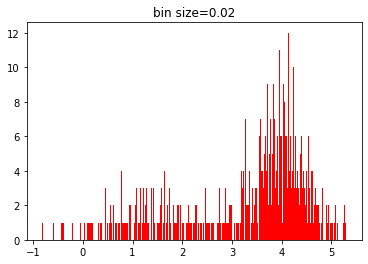
\includegraphics[width=0.5\textwidth]{h002.png}
		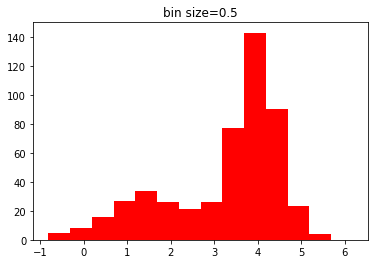
\includegraphics[width=0.5\textwidth]{h05.png}\end{figure} \begin{figure}[H]
		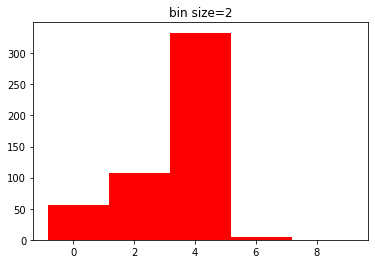
\includegraphics[width=0.5\textwidth]{h2.png}
\end{figure}
Intuitively, we suggest that the best bin-size from the three would be 0.5. Obviously, 0.02 is too small. Fixing a bin with that bin size, we got a very low probability of having even a single sample in the bin. We are very reliant on the randomly chosen data points, and therefore get a histogram where neighbored bins vary a lot. On the other hand, we see that a bin size of 2.0 gives us a result that is too smooth. We lose information of the shape of the underlying density by generalizing too much (we put too many, almost all, data points in one bowl, leaving no space for local changes in the density function). For bin size 0.5 we seem to be about right, because we see enough structure to guess the underlying distribution, and neighbored bins still seem related to another which emphasizes our idea of an underlying continuous density. This is refered to as the Bias-Variance Problem.
	\end{subtask}
\begin{subtask}
	We compute the probability density estimates for Gaussian kernels with three different variances. Also we compute the log-likelihood of these estimates. Therefore we implement \begin{lstlisting}[language=Python]
def gaussian_kernel(data, x, sigma):
	result = 0
	for i in range(len(data)):
		result += m.exp(-(x-data[i])**2 / (2 * sigma**2))
	result = (result/(len(data) * m.sqrt(2 * m.pi * sigma**2)))
	return result

def log_likehood_gaussian(data, log_like_data, sigma):
	result = 0
	for i in range(len(log_like_data)):
		result += np.log(gaussian_kernel(data, log_like_data[i], sigma))
	return result
	\end{lstlisting}
	and calling
	\begin{lstlisting}[language=Python]
	# # settings
	data = nonParamTrain
	# plot densities
	x = np.linspace(-4,8,100)
	y = []
	for sigma in [0.03, 0.2, 0.8]:
		for i in range(len(x)):
			y.append(gaussian_kernel(data, x[i], sigma))
		plt.plot(x,y,label=str(sigma))
		plt.legend()
		y = []
	plt.show()
	
	
	# log-likehood
	for sigma in [0.03, 0.2, 0.8]:
		log_likehood_solution = log_likehood_gaussian(data, data, sigma)
		print("sigma:", sigma, "log_likehood:", log_likehood_solution)
	\end{lstlisting}
	we get the following plot of the densities, labeled with the sigma value of the Gaussian kernel:
	\begin{figure}[H]
		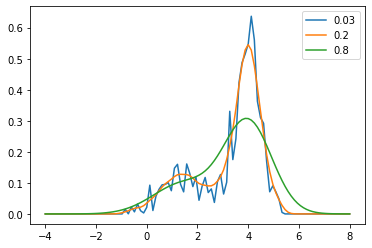
\includegraphics{3bplot.png}
	\end{figure}
and the following results for the log likelihoods:
\begin{lstlisting}
sigma: 0.03 log_likehood: -674.7279387090639
sigma: 0.2 log_likehood: -717.0216577444168
sigma: 0.8 log_likehood: -795.6632833459039
\end{lstlisting}
Interpretation: the bigger the log-likelihood number, the higher the probability that our data actually has the underlying density. Only taking this into account, we should decide on sigma=0.03. One could argue though, that the density for sigma=0.03 is not very smooth. So if we want to take this 'smoothness' into account without losing too much likelihood, we could select sigma=0.2 as a fair trade-off.
	\end{subtask}
\begin{subtask}
	We estimate the probability density with the K-nearest neighbors method with $K=2,8,35$. In the plot we see that the bigger K gets, the smoother our estimate gets. This is, once again, because for big K we sum up a big amount of data points and therefore we 'lose' information on local peaks. We wrote the function
	\begin{lstlisting}[language=Python]
	def k_nearest_neighbor(data,K,x):
		values = np.column_stack((data, data))
		values[:,0] = abs(values[:,0] - x)
		values = values[values[:,0].argsort()]
		result = values[K-1,0]
		v=2*result
		return (K / (v * len(data)))
	\end{lstlisting}
	and called with 
	\begin{lstlisting}[language=Python]
	x = np.linspace(-4,8,400)
	y = []
	for K in [2, 8, 35]:
		for i in range(len(x)):
			y.append(k_nearest_neighbor(data,K,x[i]))
		plt.plot(x,y,label="K="+ str(K))
		plt.legend()
		y = []
	plt.show()
	\end{lstlisting}
	we get the following graphs:
	\begin{figure}[H]
		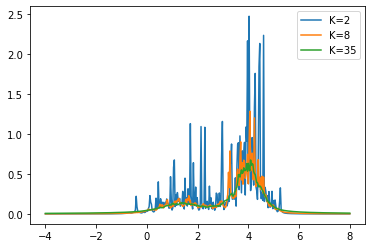
\includegraphics{3cplot.png}
	\end{figure}
	\end{subtask}
\end{task}
	
\end{document}